\section{Parameterbestimmung}
Um die Parameter des Prozesses zu bestimmen, sind zwei Sprungantworten
aufgezeichnet zu verschiedenen Stellungen der Wirbelstrombremse.

\subsection{Parameter aus Messdaten lesen}
Für die Bestimmung der Parameter aus den Messdaten ist das
Wendetangentenverfahren angewandt. Dies liefert die folgenden 
Ergebnisse.

\subsubsection{Parameter für $G_1(s)$}
Aus den Messkurven lassen sich folgende Zeitkonstanten herleiten
\[
	t_0 = 3.25\si{\second},
	\quad t_{T_u} = 3.33\si{\second},
	\quad t_{T_g} = 3.722\si{\second}
\]
\[ \Rightarrow T_u = (t_{T_u} - t_0) = 0.08\si{\second} \]
\[ \Rightarrow T_g = (t_{T_g} - t_{T_u}) = 0.392\si{\second} \]
Aus diesen Zeitkonstanten sind nun die Parameter $T_1$, $T_d$ und $K_p$
zu bestimmen mit der Tabelle zum Wendetangentenverfahren mit Ordnung 2.
\[ \Rightarrow T_1 = 0.1727\si{\second} \]
\[ \Rightarrow T_d = 0.0394\si{\second} \]
\[ \Rightarrow K_g = 245.5\si[per-mode=fraction]{\per\minute\per\volt} \]

\subsubsection{Parameter für $G_2(s)$}
Aus den Messkurven lassen sich folgende Zeitkonstanten herleiten
\[
	t_0 = 3.76\si{\second},
	\quad t_{T_u} = 3.83\si{\second},
	\quad t_{T_g} = 4.118\si{\second}
\]
\[ \Rightarrow T_u = (t_{T_u} - t_0) = 0.07\si{\second} \]
\[ \Rightarrow T_g = (t_{T_g} - t_{T_u}) = 0.288\si{\second} \]
Aus diesen Zeitkonstanten sind nun die Parameter $T_1$, $T_d$ und $K_p$
zu bestimmen mit der Tabelle zum Wendetangentenverfahren mit Ordnung 2.
\[ \Rightarrow T_1 = 0.1269\si{\second} \]
\[ \Rightarrow T_d = 0.0402\si{\second} \]
\[ \Rightarrow K_g = 150.5\si[per-mode=fraction]{\per\minute\per\volt} \]

\subsubsection{Parameterkontrolle}
Die aus den Messdaten ausgelesenen Parameter ergaben, dass eine Diskrepanz
von Modell-Simulation und Messdaten besteht. Die Modellannahmen scheinen
grundsätzlich korrekt zu sein (PT$_2$ mit Totzeit).

\begin{figure}[h!]
	\centering
	\begin{subfigure}{0.475\textwidth}
		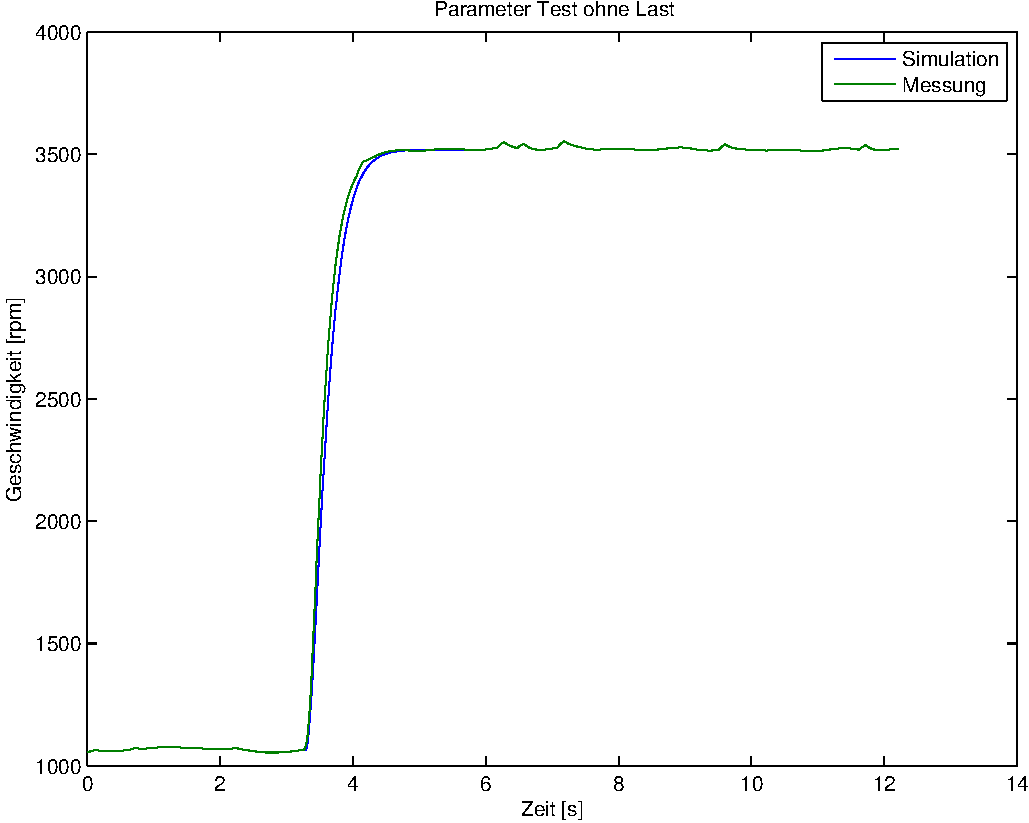
\includegraphics[width=1\textwidth]{07/parameter_test_noload.pdf}
		\caption{Ohne Bremsbelastung ($\alpha = 0$)}
	\end{subfigure}
	\begin{subfigure}{0.475\textwidth}
		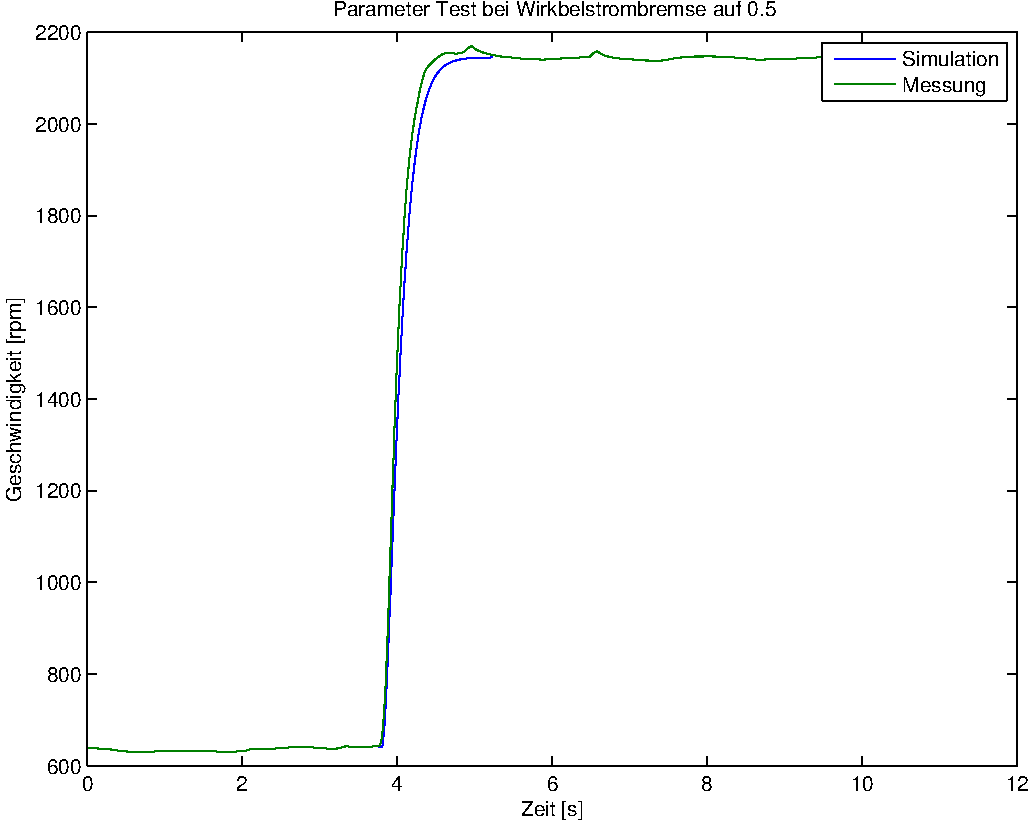
\includegraphics[width=1\textwidth]{07/parameter_test_load.pdf}
		\caption{Mit Bremsbelastung ($\alpha = 0.5$)}
	\end{subfigure}
	\caption{Vergleich der Sprungantworten von Modell und Messdaten}
\end{figure}

\subsection{Parameter empirisch ermitteln gegen Messdaten}
Die Parameter sind manuell so angepasst, dass diese ein Modell liefern, weches
den Messdaten möglichst nahe kommt in der Simulation. Hierfür ergeben sich die
folgenden Werte.

\subsection{Parameter für $G_1(s)$}
\[ T_1 = 0.1468\si{\second} \]
\[ T_d = 0.035\si{\second} \]
\[ K_g = 245.5\si[per-mode=fraction]{\per\minute\per\volt} \]

\subsection{Parameter für $G_2(s)$}
\[ T_1 = 0.1015\si{\second} \]
\[ T_d = 0.045\si{\second} \]
\[ K_g = 150.5\si[per-mode=fraction]{\per\minute\per\volt} \]

\subsubsection{Parameterkontrolle}
\begin{figure}[h!]
	\centering
	\begin{subfigure}{0.475\textwidth}
		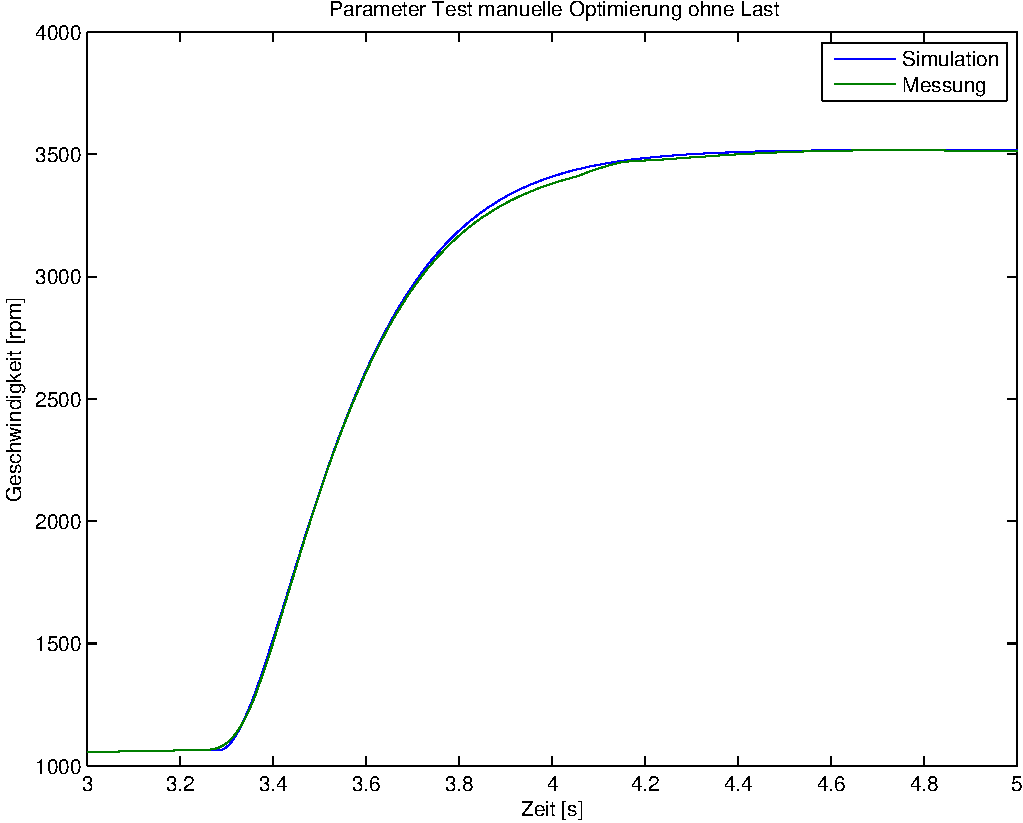
\includegraphics[width=1\textwidth]{07/parameter_test_noload_man.pdf}
		\caption{Ohne Bremsbelastung ($\alpha = 0$)}
	\end{subfigure}
	\begin{subfigure}{0.475\textwidth}
		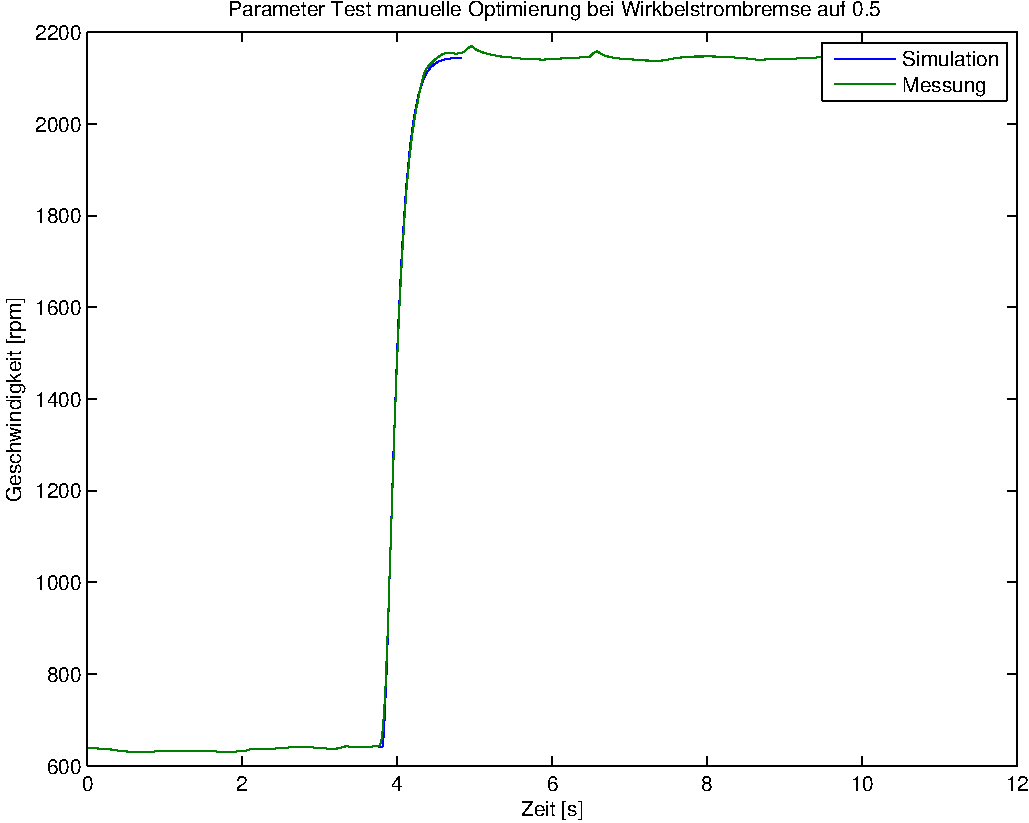
\includegraphics[width=1\textwidth]{07/parameter_test_load_man.pdf}
		\caption{Mit Bremsbelastung ($\alpha = 0.5$)}
	\end{subfigure}
	\caption{Vergleich der Sprungantworten von manuell angepasstem Modell und Messdaten}
\end{figure}

